\section{Méthodes et Outils}

\begin{frame}{Architecture}
  \begin{block}{Découpage en applications}
    {\color{darkred}\textit{authentication}}, 
    {\color{darkblue}\textit{publication}}, 
    {\color{darkgreen}\textit{home}}
  \end{block}
  
  \begin{block}{Définition des principales urls}
    \tiny
    \begin{itemize}
    \item {\color{darkred} \url{login/}}
    \item {\color{darkred} \url{logout/}}
    \item {\color{darkred} \url{signup/}}
    \item {\color{darkblue} \url{tickets/}}
    \item {\color{darkblue} \url{tickets/<int:id>/edit}}
    \item {\color{darkblue} \url{tickets/<int:id>/review}}
    \item {\color{darkblue} \url{tickets/review}}
    \item {\color{darkblue} \url{reviews/<int:id>/edit}}

    \item {\color{darkgreen} \url{/}} (\textit{news feed})
    \item {\color{darkgreen} \url{social/}}
    \item {\color{darkgreen} \url{me/}}
    \end{itemize}
  \end{block}
\end{frame}

\begin{frame}[fragile]{Les modèles}
  \begin{block}{Utilisateur}
    \begin{lstlisting}
      class User(AbstractUser):
      pass
    \end{lstlisting}    
  \end{block}
\end{frame}

\begin{frame}[fragile]{Les modèles}
  \begin{block}{Les Tickets}
    \tiny
    \begin{lstlisting}
      class Ticket(models.Model):
          title = models.CharField(max_length=128)
          description = models.TextField(max_length=248,
          blank=True)
          user = models.ForeignKey(to=settings.AUTH_USER_MODEL,
          on_delete=models.CASCADE)
          image = models.ImageField(null=True, blank=True)
          time_created = models.DateTimeField(auto_now_add=True)
    \end{lstlisting}    
  \end{block}

  \begin{block}{Les Critiques}
    \tiny
    \begin{lstlisting}
      class Review(models.Model):
          ticket = models.ForeignKey(to=Ticket, on_delete=models.CASCADE)
          rating = models.PositiveSmallIntegerField(validators=[
            MinValueValidator(0),
            MaxValueValidator(5)
          ])
          user = models.ForeignKey(to=settings.AUTH_USER_MODEL,
          on_delete=models.CASCADE)
          headline = models.CharField(max_length=128)
          body = models.TextField(max_length=8192, blank=True)
          time_created = models.DateTimeField(auto_now_add=True)
    \end{lstlisting}
  \end{block}
\end{frame}

\begin{frame}[fragile]{Les modèles}
  \begin{block}{Les Abonnements}
    \tiny
    \begin{lstlisting}
      class UserFollows(models.Model):
          user = models.ForeignKey(to=settings.AUTH_USER_MODEL,
          on_delete=models.CASCADE,
          related_name='following')
          followed_user = models.ForeignKey(to=settings.AUTH_USER_MODEL,
          on_delete=models.CASCADE,
          related_name='followed_by')
          
          class Meta:
              unique_together = ('user', 'followed_user')
    \end{lstlisting}    
  \end{block}
\end{frame}

\begin{frame}[fragile]{Les contrôleurs}
  \begin{block}{Utilisation de vues génériques}
    \tiny
    \begin{lstlisting}
      class SignupPage(generic.CreateView):
          form_class = forms.UserForm
          success_url = reverse_lazy('login')
          template_name = 'authentication/signup.html'


      class LoginPage(LoginView):
          form_class = forms.LoginForm
          template_name = 'authentication/login.html'
          next_page = reverse_lazy('signup')


      class LogoutPage(LogoutView):
          next_page = reverse_lazy('login')

    \end{lstlisting}
  \end{block}
\end{frame}

\begin{frame}[fragile]{Les contrôleurs}
  \begin{block}{Utilisation de vues basées sur des classes}
    \tiny
    \begin{lstlisting}
      class CreateTicketReview(LoginRequiredMixin, View):
          def get(self, request, id):
              ticket = get_object_or_404(models.Ticket, id=id)
              author = User.objects.get(id=ticket.user_id)
              form = forms.ReviewForm()
              
              return render(request, 'publication/ticket_review.html', {
                'ticket': ticket,
                'author': author,
                'form': form
              })

          def post(self, request, id):
              ticket = get_object_or_404(models.Ticket, id=id)
              author = User.objects.get(id=ticket.user_id)
              form = forms.ReviewForm(request.POST)
              
              if form.is_valid():
                  review = form.save(commit=False)
                  review.ticket = ticket
                  review.user = request.user
                  review.save()
                  return redirect('me')
              
              return render(request, 'publication/ticket_review.html', {
                'ticket': ticket,
                'author': author,
                'form': form
              })
    \end{lstlisting}
  \end{block}
\end{frame}

\begin{frame}[fragile]{Les vues}
  \begin{block}{Vues partielles}
    \tiny
    \begin{center}
      \fbox{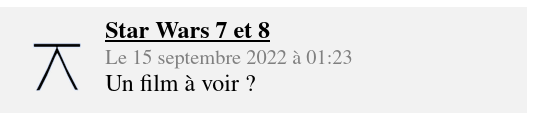
\includegraphics[scale=0.2]{img/ticket.png}}
      \fbox{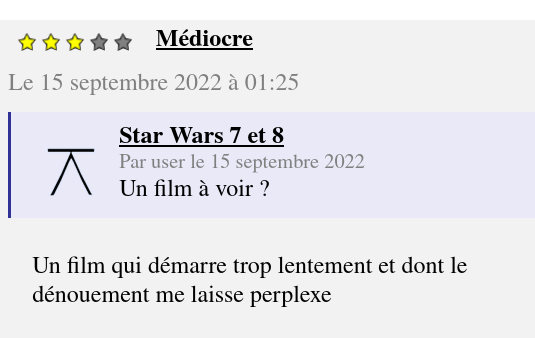
\includegraphics[scale=0.2]{img/review.png}}
    \end{center}

    \begin{lstlisting}
      
      
    \end{lstlisting}
  \end{block}
\end{frame}

\begin{frame}[fragile]{Les vues}
  \begin{block}{Vues héritées}
    \tiny
    \begin{lstlisting}{language=html}
      
      
          <!-- Code de la vue-->
      
    \end{lstlisting}
  \end{block}
\end{frame}
